\documentclass[fleqn,10pt]{wlscirep}
\usepackage[utf8]{inputenc}
\usepackage[T1]{fontenc}
\usepackage{graphicx}
\usepackage{hyperref}
\usepackage{breakcites}
\usepackage{float}
\usepackage{textcomp}
\usepackage{amsmath}
\usepackage{textgreek}
\usepackage{authblk}
\usepackage{rotating}
\usepackage{booktabs}
\usepackage{longtable}
\usepackage{pdflscape}
\usepackage{lineno}
\usepackage{xcolor}
% \usepackage[
%   style=numeric,
%   citestyle=numeric-comp,
%   backend=biber,
%   doi=true,
%   natbib=true,
%   sorting=none
% ]{biblatex}
\usepackage{scalerel,xparse}

% To be able to use emojis
\NewDocumentCommand\emojismile{}{
    \scalerel*{
        
\includegraphics{smiling-face-with-smiling-eyes_1f60a.png}
    }{X}
}

%https://www.overleaf.com/project/5f918edd1afc380001feca0d
\title{Fine-scale Twitter Big Data Reveals Neighborhood Inequalities in Mental Health Effects of High Temperatures}

\author[1,*]{Matthew Cooper}
\author[2]{Jeremiah Osborne-Gowey}
\author[3]{Zheng Liu}
\author[4]{Jie Liu}
\author[5]{Portia Adade Williams}
\author[6]{Aaron Schwartz}
\author[7]{Patrick Baylis}

\affil[1]{T.H. Chan School of Public Health, Harvard University}
\affil[2]{Environmental Studies Program, University of Colorado Boulder}
\affil[3]{Department of Geographical Sciences, University of Maryland College Park}
\affil[4]{School of Business, East China University of Science and Technology}
\affil[5]{University of Cape Town}
\affil[6]{University of Colorado Boulder}
\affil[7]{University of British Columbia}
\affil[*]{Corresponding Author: mcooper@hsph.harvard.edu}


\begin{abstract}
%Limit 150 words: https://www.nature.com/nclimate/about/content
%Actually there are lots of examples of articles with > 150 words, but I think we should keep it concise
Higher temperatures associated with climate change are expected to have major impacts on human mental health.  Indeed, traditional analyses of heat and mental health outcomes using data collected by public agencies have found strong associations between elevated temperatures and outcomes such as suicides and mental-health related hospitalizations.  However, these studies, which typically use data reported at the city or county level, have found no difference in vulnerability based on income or race.  We overturn this finding and show that there are stark differences in vulnerability using a novel data source: expressed sentiment in a quarter of a billion geolocated tweets, matched with prevailing weather as well as neighborhood economic and demographic conditions.  We find that increased temperatures worsen expressed sentiment in all areas, but that this effect is much stronger in poor and black neighborhoods.
\end{abstract}
\begin{document}

\raggedbottom
\maketitle
\thispagestyle{empty}

\section*{Main}
%Overview
Climate change is impacting many aspects of human well-being. A large body of research has explored the ongoing impacts of climate change on agricultural outcomes, economic growth, and physical health \cite{pachauri2014climate}.  However, academic and medical researchers have highlighted the relative paucity of empirical studies on the impacts of climate change on mental health \cite{Berry2018Apr, hayes_climate_2018}. While mental health is under-studied, it accounts for up 13\% of the global burden of disease, representing a major share of total human suffering \cite{Collins2011Jul}, leading to calls for more research into potential linkages between climate change and mental health \cite{Berry2018Apr, Collins2011Jul}. Researchers have begun to answer these calls, finding associations between climate disasters and post-traumatic stress \cite{Waite2017Dec, Raker2019Dec}, deteriorating environmental conditions and a sense of "ecological grief" \cite{Cunsolo2018Apr}, and linkages between higher temperatures and a variety of mental health impacts \cite{baylis_weather_2018, Mullins2019Dec, Li2020Mar, Obradovich2018Oct}.  Nevertheless, with average global temperatures projected to increase by 1.5\textdegree C within a decade \cite{allen2019technical}, more research is needed into the impacts of heat on mental health, especially on identifying the most vulnerable communities.

%Theoretical: frameworks and pathways
Researchers have proposed a number of frameworks that focus on pathways by which temperature can affect mental health \cite{Berry2018Apr, Palinkas2020Apr, BerryETAL2010}. Work on biological mechanisms emphasizes the mental health effects from dehydration and other consequences of maintaining stable body temperature in high heat \cite{Lohmus2018Jul, sadiq_impact_2019}. Additionally, recent studies find nighttime temperatures affect sleep quality, with consequences for mental health \cite{Obradovich2017May, Mullins2019Dec}. Other studies point to linkages between increased temperatures, overall physical health and increases in injuries which can have compounding consequences for exacerbate mental health issues \cite{Berry2007, WHO2007}. Finally, exposure to higher temperatures can affect productivity and income \cite{kjellstrom_impact_2016, Burke2015Nov}, leading to second-order impacts on mental health impacts and outcomes \cite{Katz1997, CohnETAL2004, BouchamaETAL2007}.

%Empirical: Heat and mental health
Results from an emerging literature indicate higher temperatures are also associated with indicators of deteriorating mental health.  Multiple studies find strong evidence that higher temperatures are associated with increases in suicides in the United States \cite{Burke2018Aug, Mullins2019Dec, Dixon2007May}. Other studies find similar relationships in locations around the world \cite{Qi2014Dec, Page2007Aug, Likhvar2011Jan}. Higher temperatures are also correlated with increased hospitalizations related to general mental health issues \cite{Obradovich2018Oct, Mullins2019Dec} and incidents related specific conditions like bipolar disorder and schizophrenia \cite{Lee2007Jan, Sung2013Feb}. Higher temperatures are also linked to increased mortality among people with mental health disorders \cite{Hansen2008Oct}.

The effects of heat exposure on mental health are relatively well established, yet results from research conducted at national scales indicate surprisingly little heterogeneity in impacts, with consequences for our understanding of who may be most or least vulnerable to heat stress and ways we plan for and adapt to changing environmental conditions. For example, a large study of temperature and suicide in the USA and Mexico found ``no significant difference in suicide response to temperature between rich and poor municipalities or counties" \cite{Burke2018Aug}. Similarly, a national study found no effect of income as modifier of the effect of temperature on suicides, emergency department visits, or self-reported mental health status across the USA \cite{Mullins2019Dec}. A major challenge for these studies, however, is their reliance on data from public health agencies, data which is typically aggregated to the municipality or county level.  As a consequence, these studies are often restricted to between-county metrics of vulnerability and cannot take into account neighborhood effects.

Findings from large-scale studies of relatively uniform vulnerability to heat are surprising given minority groups and poorer people are more likely to be exposed to undesirable temperatures and otherwise less able to mitigate the effects of higher heat. For example, people from poorer socio-economic backgrounds are more likely to work outside rather than indoors \cite{Gubernot2014Oct}, more likely to rely on public transportation, bicycling, or walking instead of commuting in their own air-conditioned car \cite{Karner2015Dec}, and more likely to live in housing that is less insulated with poorer quality or no air-conditioning \cite{Samuelson2020Jun}. Thus, there are strong reasons to expect heterogeneities in the impact of heat on mental health outcomes, with these heterogeneities in vulnerability being more pronounced within cities rather than between cities. Indeed, other studies find large differences in vulnerability between neighborhoods for a variety of impacts of heat on physical health  \cite{Belanger2015Mar, Uejio2011Mar} and mental health for other types of climate shocks like hurricanes \cite{ferre2019hurricane, Gruebner2015Jun}.

While public health data on mental health outcomes is not available at the neighborhood scale, spontaneous, in situ data from the social media platform Twitter can provide an important, inexpensive and timely indicator of mental health at extremely precise spatial and temporal scales. Many studies use the mood expressed in social media as an indicator of mental health \cite{Edo-Osagie2020Jul, Sinnenberg2016Dec}. For example, studies have used Twitter data to identify the onset of Post Traumatic Stress Disorder (PTSD) in individuals even before their formal diagnosis \cite{Reece2017Oct}. Similar methods applied to posts on Facebook can predict the onset of depression \cite{Eichstaedt2018Oct}. In London, day-to-day changes in mental health indicators derived from the text of Tweets were associated with changes in mental health crisis episodes \cite{Kolliakou2020Feb}. Across the USA, more positive Tweets are associated with a variety of metrics of human well-being \cite{Mitchell2013May}. Finally, the mood expressed in Tweets has been strongly associated with local weather conditions \cite{baylis_weather_2018, hannak_tweetin_2012} and been used as evidence to support the temperature-suicide relationship \cite{Burke2018Aug}. Thus, posts on Twitter provide an indicator of mental health at fine enough spatial scales to examine neighborhood effects on vulnerability to higher temperatures. We therefore draw on a data set of 243 million geolocated tweets from across the continental United States and covering the period 2009-2019, each paired local weather and neighborhood conditions, to explore how neighborhood conditions affect the relationship between heat and mental heath.

\section*{Results}

\subsection*{Overall Effect}
We examine the relationship between the sentiment expressed in tweets and the prevailing Wet Bulb Globe Temperature (WBGT), a temperature metric that accounts for dry-bulb temperature, humidity, wind speed, and solar radiation to more accurately describe the effects of heat on the human body \cite{budd2008wet}. Controlling for a variety of fixed effects across all Tweet, we find higher temperatures are associated with lower sentiment (i.e., worsening mood; See Fig. \ref{fig:wbgt}).  Sentiment is highest at 5\textdegree C WBGT (a dry bulb temperature typically around 12\textdegree C/54\textdegree F) with the largest declines in sentiment between 20\textdegree -25\textdegree C WBGT (dry bulb 29\textdegree-36\textdegree C/84\textdegree-97\textdegree F). Sentiment also declines with colder temperatures (below 5\textdegree C WBGT), although only slightly. We ran models using multiple measures of sentiment and find similar results and patterns across all sentiment measures (see Supplement).

\begin{figure}[H]
  \centering
  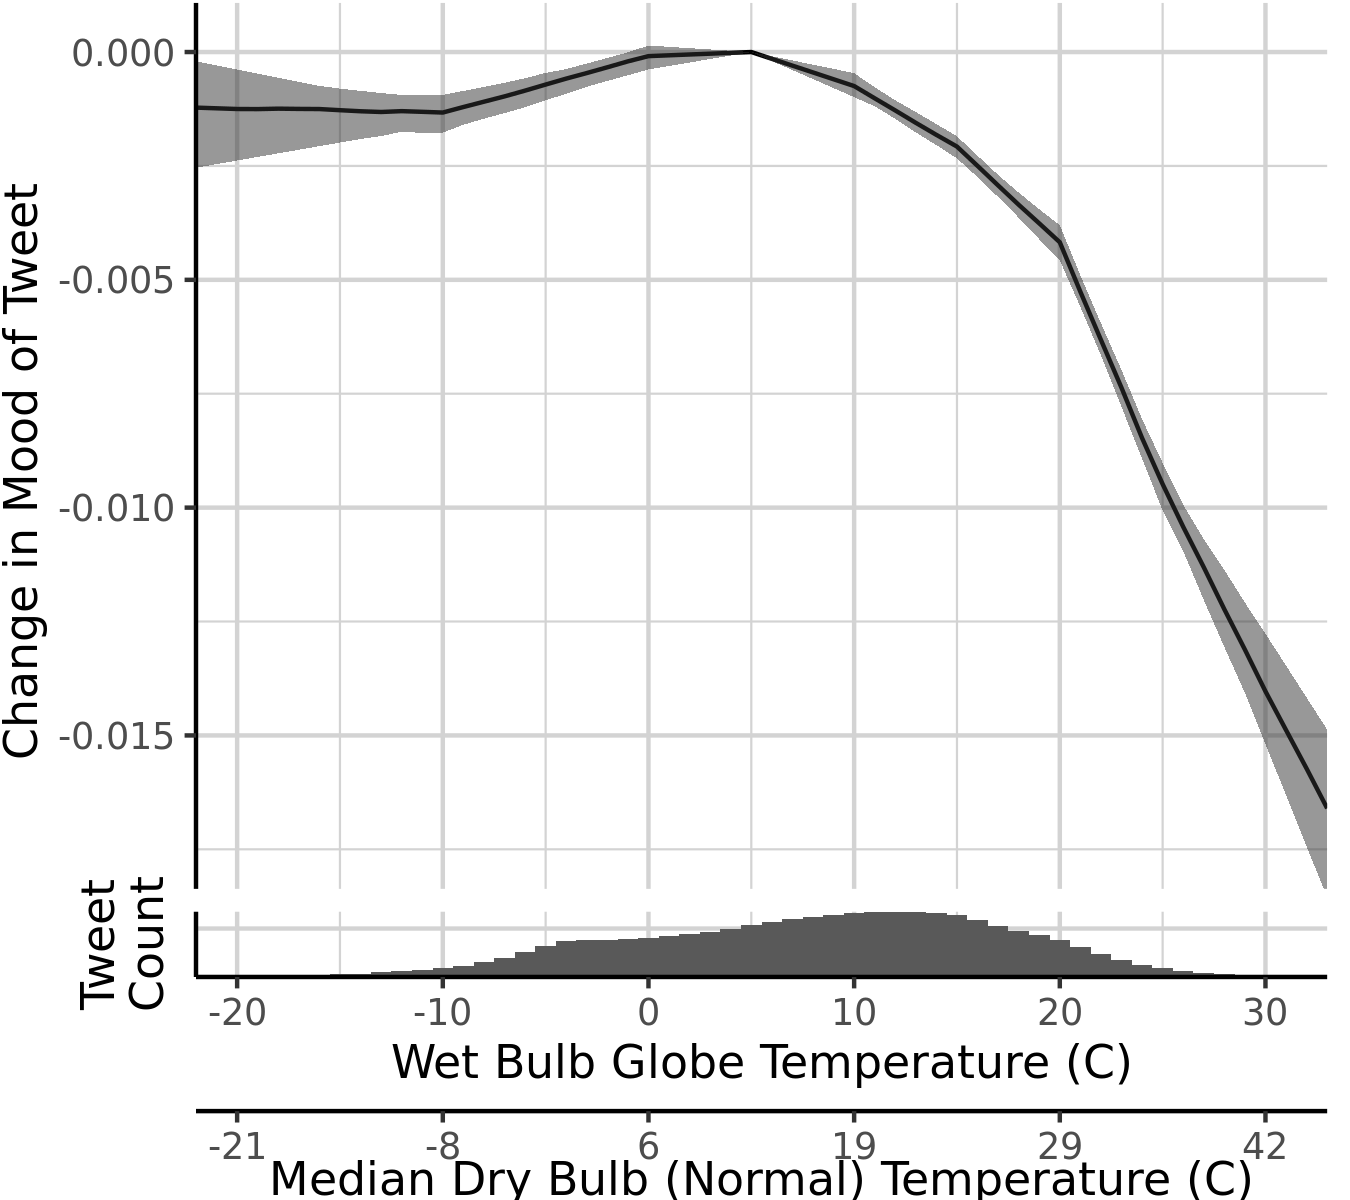
\includegraphics[width=0.5\linewidth]{../res/wbgt.png}
  \caption{Relationship between Wet Bulb Globe Temperature (WBGT) and sentiment from text in Tweets.  As temperatures increase above 5\textdegree C WBGT, sentiment rapidly declines.}
  \label{fig:wbgt}
\end{figure}

We find median neighborhood income strongly moderates the relationship between temperature and sentiment (see Fig \ref{fig:hetero}, panel A), with large differences in sentiment between the poorest and wealthiest neighborhoods. As temperatures increase to a modest 20\textdegree C WBGT (29\textdegree C/84\textdegree F), sentiment increases in the wealthiest neighborhoods (95th income percentile) but decreases in the median and lowest income neighborhoods. The wealthiest neighborhoods do not see decreases in sentiment until temperatures exceed 20\textdegree C WBGT (29\textdegree C/84\textdegree F), at which point sentiment decreases relatively evenly regardless of neighborhood income percentile.

We explored the relationship between neighborhood racial group characteristics and temperature and sentiment and find the effects of heat are felt disproportionately in neighborhoods that are majority black (see Fig \ref{fig:hetero}). Relative to an optimum temperature of 5\textdegree C WBGT (12\textdegree C/54\textdegree F), as temperatures increase to 30\textdegree C WBGT (42\textdegree C/108\textdegree F), the sentiment of tweets in majority black neighborhoods decrease four times as much as the sentiment of people in other neighborhoods. Additionally, at modest to moderate temperatures of 10\textdegree C WBGT (19\textdegree C/66\textdegree F) to 25\textdegree C WBGT (36\textdegree C/97\textdegree F), people in majority Hispanic neighborhoods have slightly lower sentiment than people in majority white or other neighborhoods, although this gap narrows at higher temperatures.

Exploring the combined effects of neighborhood percent minority race and income in moderating the impacts of heat on mental health, we find separate effects for these two variables (see Supplement). In other words, neither neither percent minority population nor income alone account for the heterogeneity in vulnerability as neighborhoods that are both poorer and higher percent black are more affected by heat than than neighborhoods that are just poorer or higher proportion black.

\begin{figure}[H]
\centering
  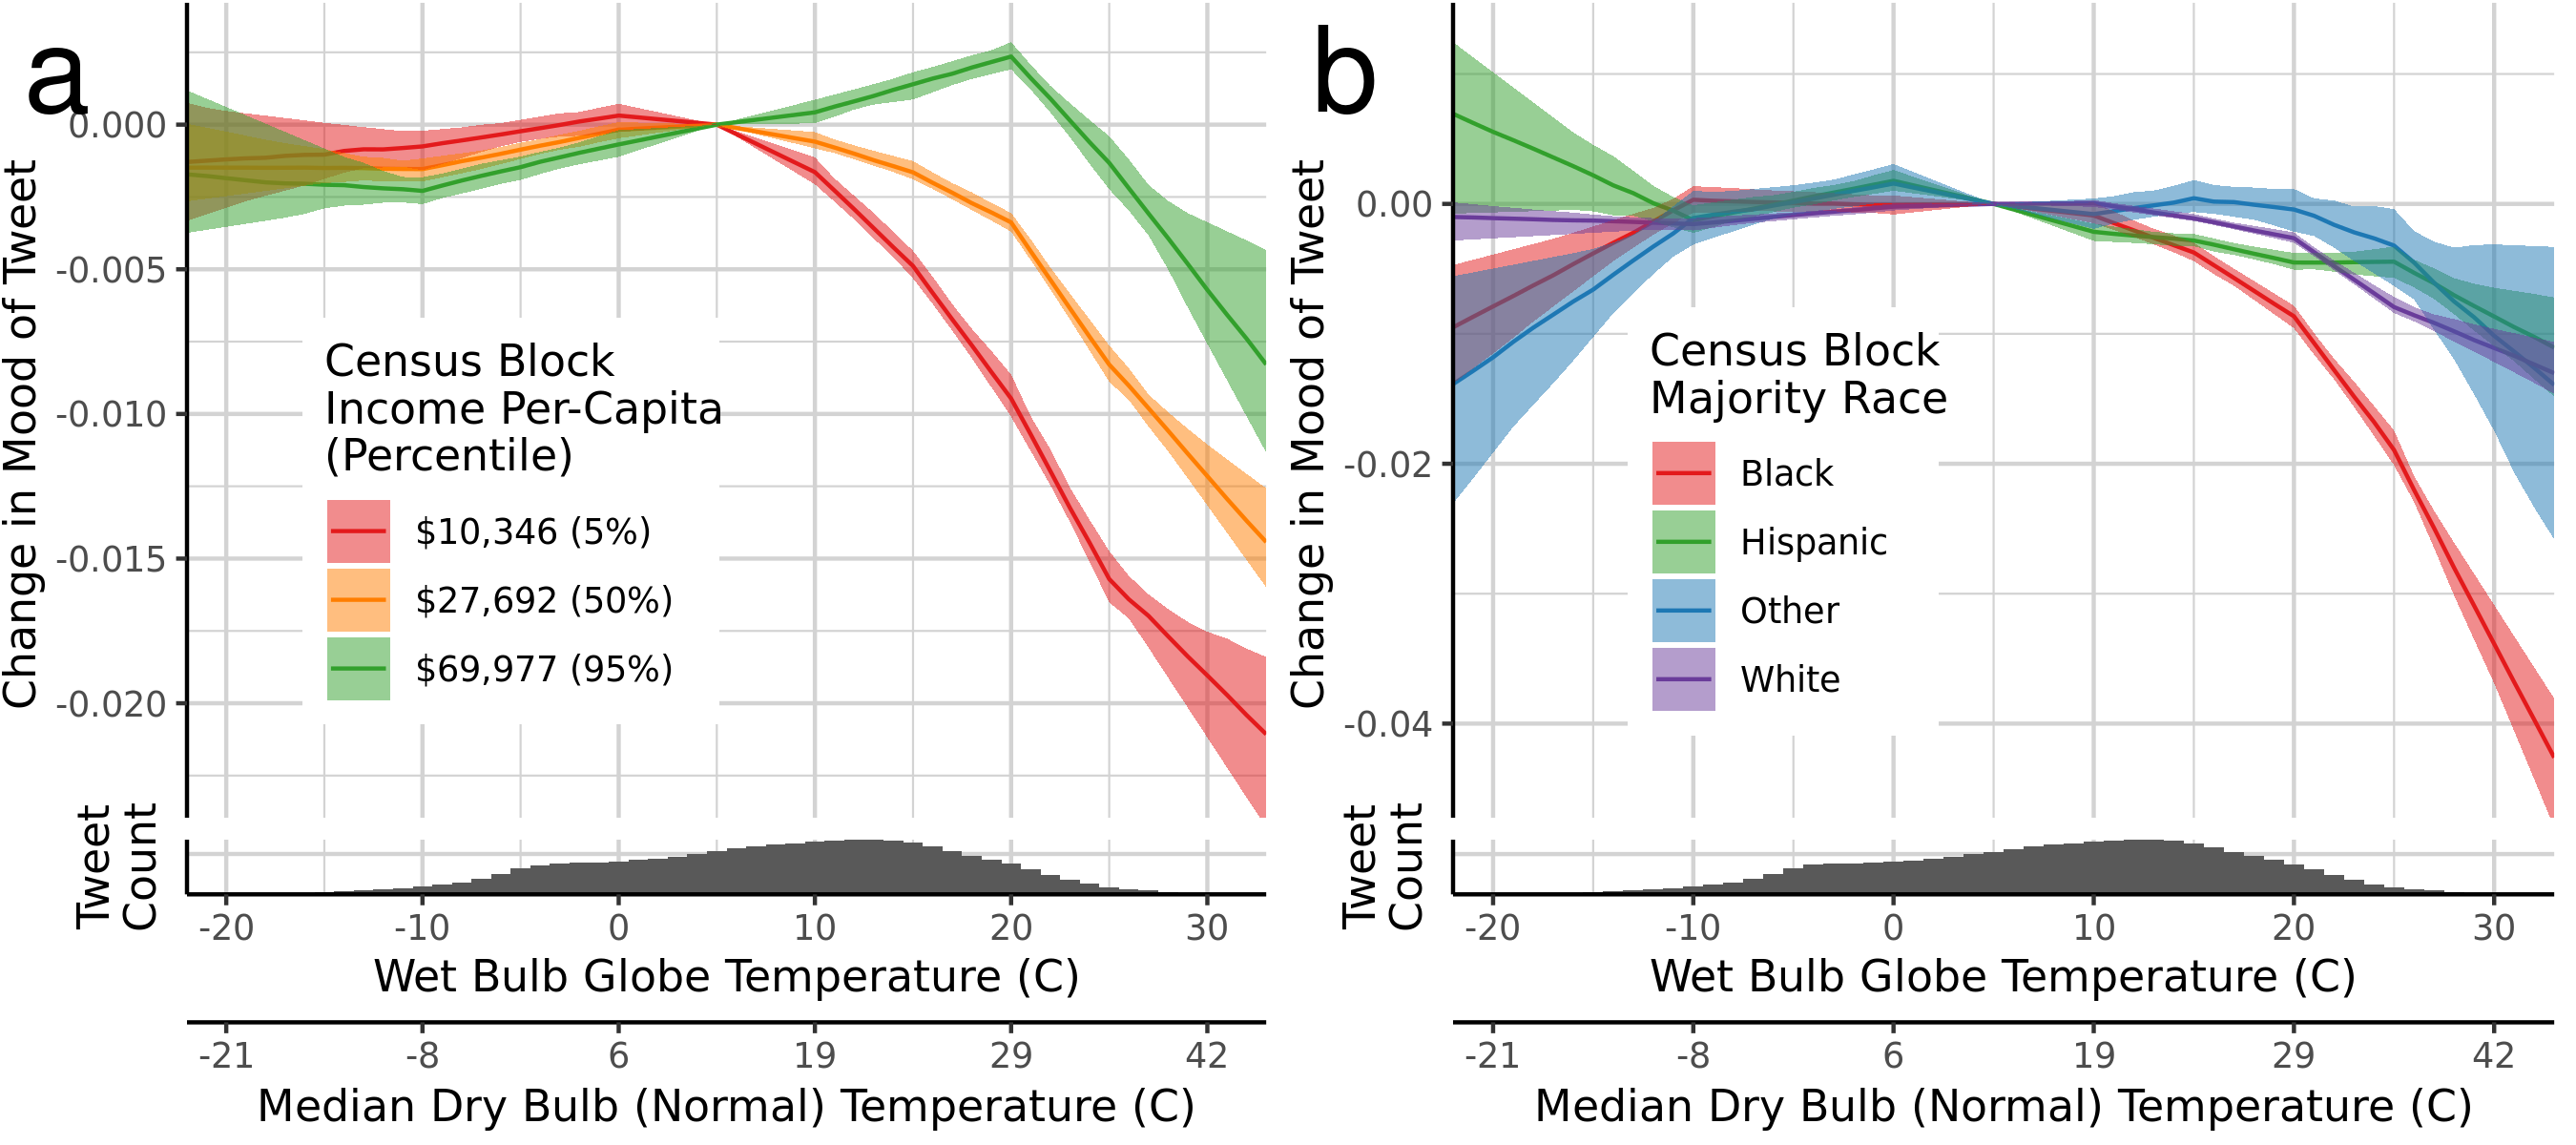
\includegraphics[width=\linewidth]{../res/wbgt_combined.png}
    \caption{Effect of changes in wet-bulb globe temperature on expressed sentiment relationship as moderated by neighborhood income (a) and race (b).}
\label{fig:hetero}
\end{figure}


\subsection*{Sentiment Comparison With Other Events}
Expressed sentiment is a widely used metric to assess mental health and well-being on social media.  While a variety of related metrics can be used to quantify sentiment, we use the VADER metric that was specifically designed for microblogs like Twitter \cite{hutto2014vader}.  To give context to this novel metric, we compare the impacts of heat waves, defined as a change from 5\textdegree C WBGT (12\textdegree C/54\textdegree F) to 25\textdegree C WBGT (36\textdegree C/97\textdegree F), to two other changes that have large impacts on sentiment (See Fig. \ref{fig:compare}).  First, we examine the change in average sentiment from Saturday to Monday, the highest and lowest days for Twitter sentiment as well as other mental health metrics, such as suicide rates \cite{CDC2021}.  We also examine the decrease in sentiment associated with one of the most expensive hurricanes in the last decade in the United States: Hurricane Sandy.  Specifically, we compare the mean sentiment of counties affected by Sandy on the week after landfall to the mean sentiment for the week previous.  Hurricanes like Sandy are associated with mental health effects including Post-Traumatic Stress Disorder (PTSD) \cite{Schwartz2017Aug, Schwartz2018May}, and similar disasters have been associated with subsequent increases in suicides \cite{Krug1998Feb}.

\begin{figure}[H]
  \centering
  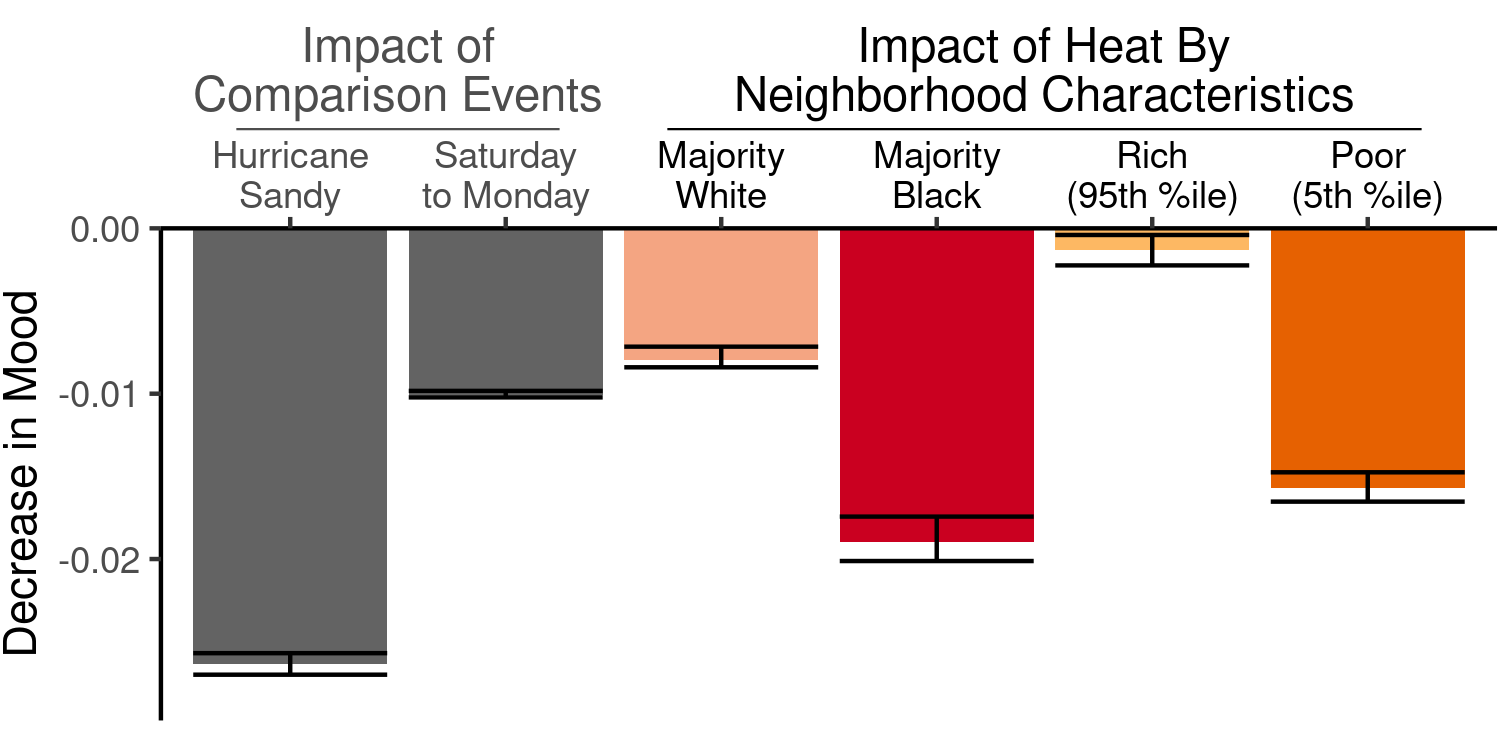
\includegraphics[width=0.66\linewidth]{../res/comparison_plot.png}
  \caption{Decline in sentiment during a heat wave across several different neighborhoods, compared with other impacts on sentiment, such as major hurricanes, as well as the weekly variation in sentiment from the peak on Saturday to the low on Monday.}
  \label{fig:compare}
\end{figure}

We find that the impacts of heatwaves on sentiment in rich and majority white neighborhoods are less than the average weekly change in sentiment from Saturday to Monday, but the effects of heat waves on majority black or poor neighborhoods are much greater than the average weekly change in sentiment.  Additionally, the impacts of heat waves on more vulnerable neighborhoods are close in severity to the impact of a major hurricane.

\subsection*{Effects by Combined Statistical Area}

To further explore our findings, we examine the impact of heat on sentiment and sentiment inequalities by Combined Statistical Areas (CSAs) and Metropolitan Statistical Areas (MSAs) with over 1 million people (hereafter: cities).  We examine the impacts of heat alone, as well as the change in size of the gap in sentiment scores between both poor and rich neighborhoods and black and non-black neighborhoods.  For our metric of inequality, we show the size of the gap in sentiment as temperatures increase from optimum temperatures of 5\textdegree C WBGT (12\textdegree C/54\textdegree F) to 30\textdegree C WBGT (42\textdegree C/108\textdegree F).

Examining the effects of heat on sentiment by city, we find that heat is associated with worsened sentiment in 83.6\% of cities, and the effect is significant in 35.3\% of those.  In no cities does heat significantly increase sentiment, and heat affects sentiment in cities across the US, from Florida to New England to California.

We find that heat increases inequalities in sentiment across income groups for 68.9\% of cities, with 35.7\% of these having a statistically significant effect.  Cities with a significantly unequal effect were found in the south, Midwest, northeast, northwest, and southwest, although they were most common in the mid-Atlantic region.  Additionally, many cities in the southwest had an inverted effect, where higher temperatures actually narrowed the gap in sentiment between rich and poor neighborhoods, including Denver and Oklahoma City, which had a statistically significant inverted effect.

Because we found a much stronger effect of temperature on sentiment in majority black neighborhoods compared to other ethnic groups, we also examined increases in sentiment gaps between neighborhoods in the 95th percentile for black population (77.2\% black) and neighborhoods in the 5th percentile for black population (0\% black).  We excluded cities with a black population less than 5\% of the total population.  We found increasing inequalities in sentiment for more black neighborhoods in 64.7\% of cities, with a significant effect in 21.2\% of those (7 cities).  Additionally, three sunbelt cities had a significant inverted effect.  The patterns of inequalities in the impacts of heat on sentiment by race were similar to inequalities by income: cities with large and significant inequalities were found the mid-Atlantic and Midwest.

\begin{figure}[H]
\centering
  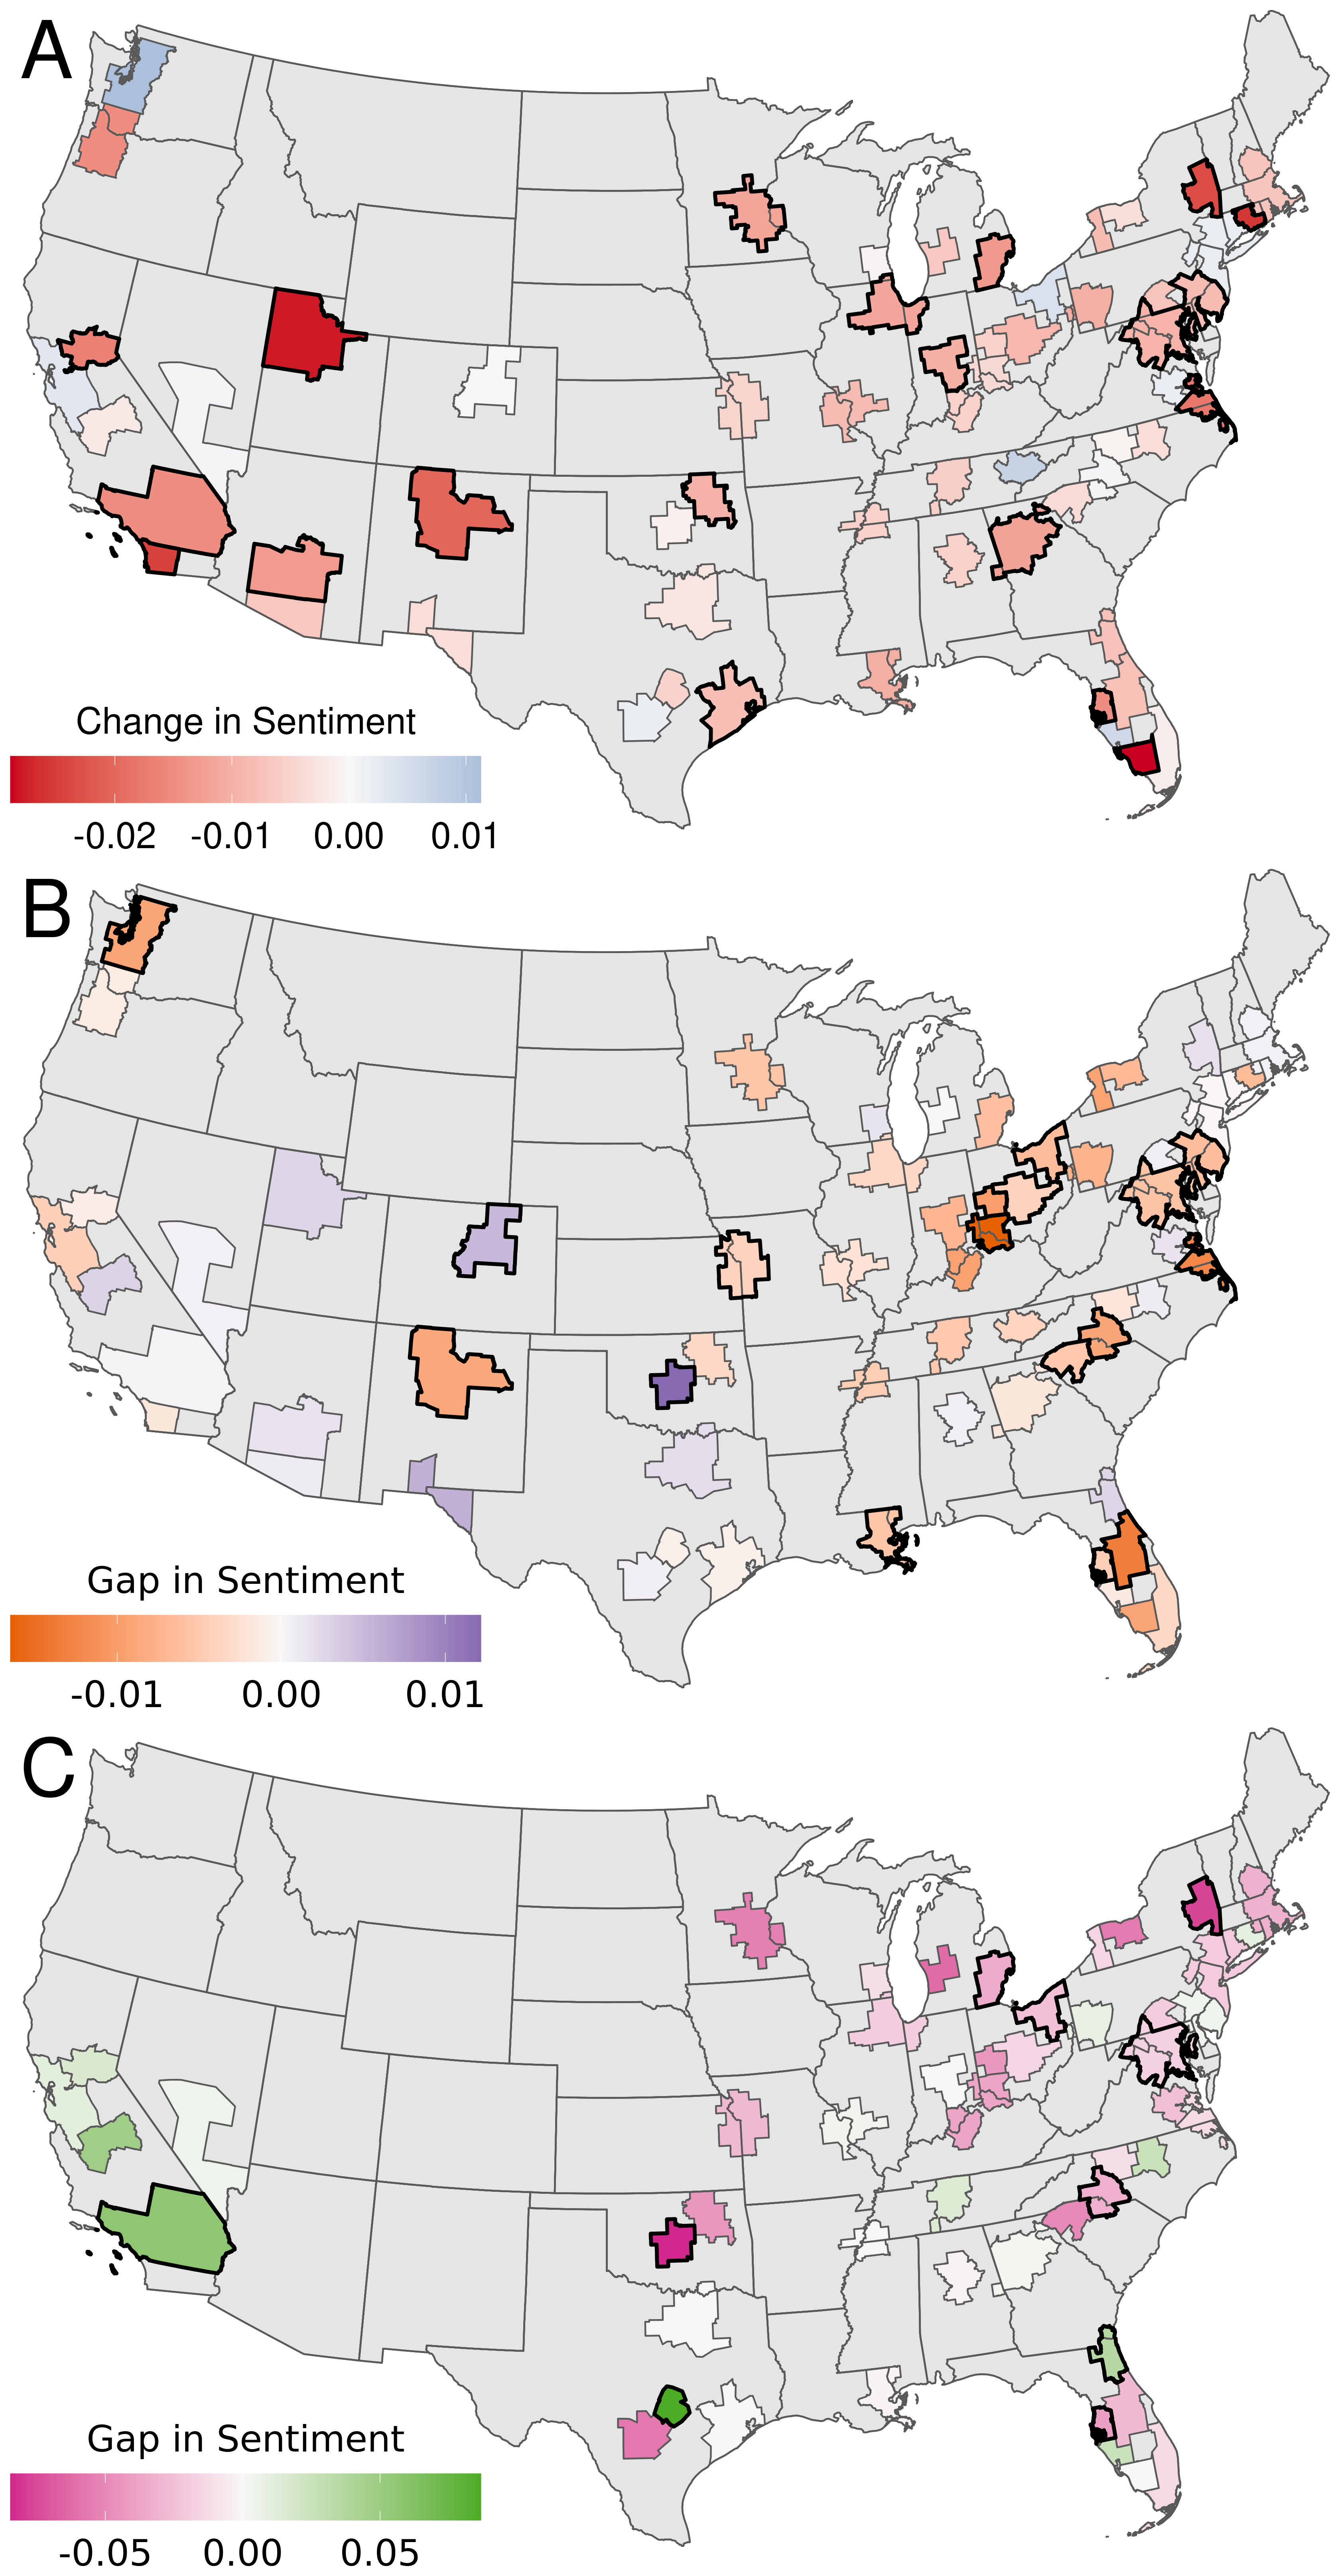
\includegraphics[width=0.5\linewidth]{../res/map_combined.png}
  \label{fig:map}
    \caption{Figure (a) shows the change in sentiment for a 25-degree increase in WBGT for cities with a population of over 1 million.  Figures (b) and (c) show inequalities in impacts of temperature on sentiment for cities with over 1 million people.  The value shown is the predicted change in the size of the gap in VADER score as temperatures increase from 5\textdegree C WBGT to 30\textdegree C WBGT between the 5th and 95 percentile for income (a) and the 95th and 5th percentile for percent black (b).  Cities with a statistically significant effect ($p < 0.05$) are outlined in black.  For racial inequalities (b), only cites where black people make up $> 5\%$ of the population are included.}
\end{figure}

\section*{Discussion}
% Benefits of twitter data/overview of findings
We found that twitter data offers significant advantages for observing environmental effects on human well-being due to its very fine spatio-temporal resolution.  We were able to pair each tweet with the local temperature at the time of the tweet, and found a clear association between heat and worsened sentiment.   Moreover, we were able to show heterogeneities in vulnerability by neighborhood characteristics, overturning previous findings that found no heterogeneities at the county level \cite{Burke2018Aug, Mullins2019Dec}.

% Sentiment is a fuzzy indicator but we have BIG DATA
One limitation of data from twitter is that a tweet is not a precise measurement of a discrete mental health outcome and only provides a rough indicator a user's mental state based on the vocabulary in the tweet.  Moreover, while sentiment analysis algorithms have gotten increasingly sophisticated at estimating the mood in a body of text, a user's expressed sentiment in a tweet is highly variable and is mostly affected by factors like current events and the user's personal life, with local weather conditions having only a small impact.  We overcome this limitation by using an extremely large data set of 243 million tweets, allowing us to control for a wide variety of spatial and temporal effects to estimate population-level changes in sentiment in relation to the weather.

% Compare weekly changes in sentiment to weekly changes in suicides
We found that the change from optimum temperature of 5\textdegree C WBGT (12\textdegree C/54\textdegree F) to a heatwave of 25\textdegree C WBGT (36\textdegree C/97\textdegree F) is associated with an overall decrease in the VADER sentiment score of 0.01.  This is similar to the degree of change in sentiment over the course of a week from a Monday nadir (0.1268) to a Saturday peak (0.1372), a weekly change associated with a increase in suicides of 23\% over the course of the study period \cite{CDC2021}.  Thus, while research on linkages between sentiment and other mental health outcomes like suicides and hospitalizations is still nascent, there are clear similarities in patters of sentiment and suicides at some time scales.  Moreover, like sentiment, suicides are affected by higher temperatures.  Thus, while twitter sentiment is the only mental health indicator available at fine enough spatial and temporal scales to examine neighborhood effects, these changes in sentiment are representative of real human suffering, and are also very likely indicative of medical outcomes like suicides and hospitalizations, although this analysis cannot speak to those outcomes specifically.

% Discuss the NOVELTY: quote Burke and Mullins, refute their interpretations, people have said XX, but we have shown ~XX.
% Variations in vulnerability also indicates ADAPTATION
Previous work conducted with county-scale data found no heterogeneities in mental health vulnerability by income.  Such analyses have led to conclusions that (1) the mental health effects of climate change will be uniform, least in developed countries, and (2) that adaptation with technologies like air-conditioning will not mitigate the mental health effects of climate change.  For example, Mullins et al. conclude that ``high-temperature events will harm mental health everywhere" and that ``individuals have not been able to successfully reduce the negative effects of higher temperatures on mental health" \cite{Mullins2019Dec}.  Contrary to these analyses, we found large heterogeneities in vulnerability by neighborhood race and income.  This suggests that the mental health effects of climate change will not be uniform and, like other impacts, will fall disproportionately on the poor and vulnerable.  More positively, it does suggest that adaptation is possible, and, for communities with infrastructure and working conditions similar those of high-income Americans, the effects of high temperatures on mental health can be largely mitigated.

% Comment on Race, why no effect on hispanics?
We found that majority black neighborhoods are much more affected by heat than neighborhoods with a majority of any other race.  This is surprising, given that Hispanics can be marginalized in both income and housing.  This finding may be because the racial category of Hispanic is more broad and encompasses many more groups with more diverse histories and income levels than black Americans, or may also be due to that fact that more marginalized and heat-vulnerable Hispanic people were more likely to tweet in the Spanish language, which we did not include our analysis.  Additionally, there are many other marginalized groups in America, particularly indigenous people, that we did not have sufficient data to examine with respect to heat and mental health.  Finally, while race is correlated with income in the US, we found that race contributed to vulnerability independently of income.  This suggests that racism and patterns of housing discrimination such as a legacy of redlining contribute to making black Americans more vulnerable to heat, event at similar levels of income.

% Interpret Spatial Analysis
In our spatial analysis, we found that heat affects sentiment in cities across the US, suggesting that higher baseline temperatures do not reduce vulnerability.   Additionally, most cities exhibited both racial and income inequalities in the vulnerability of mental health to heat, although the southwest had the weakest inequalities and an occasional inverted effect.  While unusual patterns of heat impacts in the southwest could suggest that heat inequality is related to environmental factors such as humidity, this is unlikely because we used Wet Bulb Globe Temperature, which accounts for how differences in humidity and wind speed affect the human body's ability to cool itself through perspiration.  Thus, this regional differences in vulnerability are likely more due to cultural or infrastructural differences than to different baseline environmental conditions.

% Connect to bigger literature on vulnerability
This study shows the importance of examining heterogeneities in vulnerability in analyses of climate change impacts, as well as the importance of measuring vulnerability at fine spatial scales.  Within in relatively wealthy nation of the United States, we find large heterogeneities in vulnerability.  This adds to the growing literature showing that the impacts of climate change will be highly unequal and disproportionately borne by the poor and marginalized \cite{Thomas2019Mar}.  Moreover, given that more impoverished neighborhoods in the United States see greater mental health impacts during heatwaves, it is likely that heat waves have a much greater mental health impact throughout the developing world, where temperatures are expected to be much greater \cite{Raymond2020May}, heatwaves are already under-counted \cite{Harrington2020Sep}, and adaptive technologies like air conditioning are more scarce \cite{Biardeau2020Jan}.

% Caveats
While these findings are robust to different model specifications and sentiment metrics, there are some caveats.  For one, we were only able to locate the tweets within the census block where the tweet was sent - we did not to infer where the person sending the tweets typically lived or where they had been.  Many low-income and black people commute during the day to work in the service sector in higher-income areas, so these results may in fact under-estimate the impacts of higher temperatures on mental health for poor and minority individuals.  Moreover, in some cases the income level of a census block may be only weakly indicative of the wealth of the people who are typically found that census block.  For example, some public spaces are estimated to have very low income levels even though people from a variety of income levels may occupy those spaces throughout the day.  Additionally, neighborhoods of young college students are also typically estimated to have low income levels, even through college students are wealthier than the average American.  Again, these issues mean we are likely under-estimating the true effect of heat on mental health for poor and black people.  A final issue with using twitter data is that, while twitter is used by more than one in five Americans, twitter users may not be representative of the general population, as they are typically younger, wealthier, and more educated \cite{Pew2020Sep}.  Nevertheless, we found a large volume of tweets across all neighborhood types.

% NCC doesnt have a "conclusion" section, but this is intended as an overall summary paragraph
While climate change will have widespread and severe impacts on human well-being, it cannot be overemphasized just how highly unevenly these impacts will be distributed.  People with more money, access to aid and infrastructure, and who belong to ethnic groups in power are less affected by climate shocks and natural disasters and more able to adapt \cite{bullard2012wrong}.  While the physical health impacts of these shocks are more visible and easy to measure, the mental health impacts of climate change are also causing severe human suffering and there is no reason to believe they will not also be highly unevenly distributed.  Thus, there are strong theoretical priors behind the hypothesis that low-income and marginalized people are more vulnerable to the mental health impacts of higher temperatures, even though previous work at coarse spatial scales had not found such an effect.  By using fine-scale twitter data, we show that there are indeed stark differences in the mental health impacts of heat among neighborhoods in the United States.  These findings have significant implications for urban planning, climate and environmental justice, and mental health.

\section*{Methods}
\subsection*{Tweets \& Sentiment}
We used data from 243 million geo-located English-language tweets from the continental United States from the years 2009 to 2019.  The Twitter data consists of publicly posted messages, or Tweets, that are short status messages users post to the platform.  We only considered users’ original content, thus did not include retweets in our analysis.  Additionally, we excluded all tweets that contained weather-related terms, to ensure that the sentiment expressed in the tweets was reflective of a user's mental state, and not a commentary on the weather.

We assessed the sentiment expressed in the tweets using the VADER (Valence Aware Dictionary for sentiment Reasoning) sentiment corpus \cite{gilbert_vader_2014}. VADER is a lexicon and rule-based sentiment analysis tool that is specifically attuned to sentiments expressed in social media because of several features, as:

\begin{itemize}
  \item Incorporating lexical features common to informal media, such as slang (``sux"), and acronyms (``lol").
  \item Negations (``\textit{not} good", ``\textit{wasn't} bad")
  \item Punctuation (``Good!!!")
  \item Word shape, such as capitalization (``The movie was AMAZING")
  \item Emoticons and emojis (``:-)", ``\emojismile")
  \item Degree modifiers (``very excellent" or ``kind of crappy")
\end{itemize} 

The VADER method yields a value for the mood of a tweet, with a score of 0 for neutral tweets, a score $> 0$ for positive-mood tweets and a score $< 0$ for negative-mood tweets.  In addition to the VADER method used in the body of this paper, we also conduct our analysis using the Hedonometer and XXXXX sentiment analysis methods, with similar results (See Supplement).

\subsection*{Weather}
We used data on local weather conditions from the North American Land Data Assimilation System (NLDAS), a gridded product developed by several collaborative institutions, including NOAA, NASA, Princeton University, and the University of Washington.  This dataset is available at an hourly temporal resolution, and at 1/8th decimal degree spatial resolution, and integrates a large quantity of observation-based and modeled data  \cite{xia_continental-scale_2012}.  For the exact hour and location of each tweet, we extracted temperature, specific humidity, air pressure, total precipitation, shortwave radiation, and wind speed.  

Because metrics of apparent temperature that take into account humidity and other factors can better account for the impacts of heat stress on human health and well-being, we calculate the Wet Bulb Globe Temperature (WBGT) at the time and location of each tweet.  WBGT is the temperature that a wet globe thermometer would read in direct sunlight, and gives a reading lower than a dry bulb temperature would show due to evaporative cooling, and can be estimated given normal temperature, relative humidity, solar radiation, and wind speed.  Because evaporative cooling is how humans cool themselves through perspiration, this temperature better indicates the heat stress that people are experiencing \cite{budd2008wet}.  Metrics like WBGT that account for the effects of humidity and other factors on heat stress have been associated with diminished economic output \cite{rao2020projections}, increased crime \cite{hu2017impact}, increased mortality \cite{chien2016spatiotemporal, armstrong2019role}, and worsened mental health outcomes \cite{vida2012relationship, ding2016importance}.

Using temperature, specific humidity, and pressure, we derived relative humidity using methods described by  \cite{bolton_computation_1980}.  We then calculated the WBGT using the formula described by \cite{heo2019comparison}.

Throughout the paper, we give the dry bulb temp for reference as the mean value across our data set for a given wet bulb temp.

\subsection*{Socio-Econoimc Data}
We used data from the American Community Survey (ACS) administered by the US Census to estimate income levels and the racial composition of neighborhoods where tweets were located.  Data was at the level of the census block group, the smallest unit for which the US Census releases public data. Following Census categories, we report racial characteristics of neighborhoods as majority population of four broad racial categories - non-Hispanic black, non-Hispanic white, Hispanic of any race, and other, which includes Native American, multi-racial, Asian-American and Pacific Islander. 

ACS data is released to cover five-year periods.  We therefore matched each tweet with census block group data from the year at the middle year of each survey's five-year range.  For example, tweets from 2014 were matched to data from the 2012-2016 ACS.  Because the most recent available ACS was from 2014-2018, all tweets from year years greater than 2016 were matched to this dataset.  Data was downloaded from the IPUMS NHGIS service provided by the University of Minnesota.

Mean annual income per capita is provided by the ACS, and we standardized this variable so that the values for each year were in 2019 dollars.  For racial categories, we combined the various categories provided by the ACS into four racial groups: non-Hispanic white, non-Hispanic black, Hispanic of any race, and an "other" category for non-Hispanic people who were neither black nor white, such as Asian, Native American, or mixed-race people.

In this paper, we give income and racial percentiles based on the observed percentiles across all tweets in our data set.
    
\subsection*{Modeling}
We assessed how expressed sentiment is affected by Wet Bulb Globe Temperature using segmented regressions, controlling for precipitation, and shortwave solar radiation (sunshine), as well as the following spatio-temporal fixed effects: the day of the week, the time of day, the day of the year, the year, the month, and the county.  

Our initial model (for Fig. \ref{fig:wbgt}) takes the following form:

\begin{equation}
    y = \beta_0 + f_t(t) + \beta_p p + \beta_s s + \Phi + \epsilon
    \label{mod:1}
\end{equation}

Where $y$ is the sentiment of a tweet, $t$ is the wet bulb globe temperature at the hour of the tweet, $p$ is a binary variable indicating whether it rained at the hour of the tweet, $s$ is the income shortwave radiation, or sunshine, in $W/m^2$, at the hour of the tweet, $\Phi$ is the spatio-temporal fixed effects, $\epsilon$ is the normally-distributed errors, and $f_t$ represented the segmented regression for $t$, with knots at -10\textdegree, 0\textdegree, 5\textdegree, 10\textdegree, 15\textdegree, 20\textdegree, and 25\textdegree C WBGT.  We estimate the 95\% confidence interval of our models using 80-fold bootstrapping.  

To examine how income and racial groups moderate the effect of heat on sentiment, we extend our model to the following form:

\begin{equation}
    y = \beta_0 + f_t(t) + f_{mt}(m t) + \beta_p p + \beta_{mp} m p + \beta_s s + \beta_{ms} m s + \Phi + \epsilon
    \label{mod:2}
\end{equation}

Where $m$ is either the log-transformed average income in the census block where the tweet originated, or a dummy variable for the four racial categories.  We specify alternative models where income is a dummy variable in three bins, and were race is a continuous variable for the percent of a census block population that is white These alternative specifications yield similar results.  We also examine the effects of rainfall and sunshine on sentiment by income and race.  These alternative specifications and analysis of rainfall and sunshine effects are available in the Supplement.

For our analyses by city, we run models with a similar form to Model \ref{mod:2}, including the same fixed effects, although we fit a linear effect for $f_t()$.  Additionally, for exploring the vulnerability of black americans, we use a continuous variable for $m$ indicating the percentage of a neighborhoods population that is black.  Finally, because we are not accounting for non-linearities in $f_t()$, we exclude tweets with a WBGT of less than 5\textdegree C, as our initial analysis showed that this is the temperature at which sentiment peaks.

\section*{Acknowledgements}
%Official SESYNC wording
This work was supported by the National Socio-Environmental Synthesis Center (SESYNC) under funding received from the National Science Foundation DBI-1639145.  Additionally, computational resources for this project were provided for the Microsoft Azure cloud by Microsoft's AI for Earth program.

This data came from Twitter via the University of Vermont’s (UVM) agreement with Twitter to access its streaming API - colloquially referred to as the Decahose.  The UVM special agreement with Twitter allows for access to this data for research and analysis purposes and we have complied with all the terms of service for Twitter and UVM. 

%\printbibliography
\bibliography{TextDataClimateShocks}

\section*{Author Contributions}
Author contributions: M.W.C., J.O.-G., A.S. and P.B. designed the research and modeling strategy; A.S. provided data; M.W.C and Z.L. prepared data; M.W.C. analyzed data; and M.W.C., J.O.-G., J.L., and P.A.W. wrote the paper.

\noindent This paper was the result of a SESYNC graduate pursuits project co-lead by M.W.C. and J.O.-G.

\end{document}
